\documentclass[journal,12pt,twocolumn]{IEEEtran}
%
\usepackage{setspace}
\usepackage{gensymb}
%\doublespacing
\singlespacing

%\usepackage{graphicx}
%\usepackage{amssymb}
%\usepackage{relsize}
\usepackage[cmex10]{amsmath}
\usepackage{siunitx}
%\usepackage{amsthm}
%\interdisplaylinepenalty=2500
%\savesymbol{iint}
%\usepackage{txfonts}
%\restoresymbol{TXF}{iint}
%\usepackage{wasysym}
\usepackage{amsthm}
\usepackage{iithtlc}
\usepackage{mathrsfs}
\usepackage{txfonts}
\usepackage{stfloats}
\usepackage{steinmetz}
%\usepackage{bm}
\usepackage{cite}
\usepackage{cases}
\usepackage{subfig}
%\usepackage{xtab}
\usepackage{longtable}
\usepackage{multirow}
%\usepackage{algorithm}
%\usepackage{algpseudocode}
\usepackage{enumitem}
\usepackage{mathtools}
\usepackage{tikz}
\usepackage{circuitikz}
\usepackage{verbatim}
\usepackage{tfrupee}
\usepackage[breaklinks=true]{hyperref}
%\usepackage{stmaryrd}
\usepackage{tkz-euclide} % loads  TikZ and tkz-base
%\usetkzobj{all}
\usetikzlibrary{calc,math}
\usetikzlibrary{fadings}
\usepackage{listings}
    \usepackage{color}                                            %%
    \usepackage{array}                                            %%
    \usepackage{longtable}                                        %%
    \usepackage{calc}                                             %%
    \usepackage{multirow}                                         %%
    \usepackage{hhline}                                           %%
    \usepackage{ifthen}                                           %%
  %optionally (for landscape tables embedded in another document): %%
    \usepackage{lscape}     
\usepackage{multicol}
\usepackage{chngcntr}
%\usepackage{enumerate}

%\usepackage{wasysym}
%\newcounter{MYtempeqncnt}
\DeclareMathOperator*{\Res}{Res}
%\renewcommand{\baselinestretch}{2}
\renewcommand\thesection{\arabic{section}}
\renewcommand\thesubsection{\thesection.\arabic{subsection}}
\renewcommand\thesubsubsection{\thesubsection.\arabic{subsubsection}}

\renewcommand\thesectiondis{\arabic{section}}
\renewcommand\thesubsectiondis{\thesectiondis.\arabic{subsection}}
\renewcommand\thesubsubsectiondis{\thesubsectiondis.\arabic{subsubsection}}

% correct bad hyphenation here
\hyphenation{op-tical net-works semi-conduc-tor}
\def\inputGnumericTable{}                                 %%

\lstset{
%language=C,
frame=single, 
breaklines=true,
columns=fullflexible
}
%\lstset{
%language=tex,
%frame=single, 
%breaklines=true
%}

\begin{document}
%


\newtheorem{theorem}{Theorem}[section]
\newtheorem{problem}{Problem}
\newtheorem{proposition}{Proposition}[section]
\newtheorem{lemma}{Lemma}[section]
\newtheorem{corollary}[theorem]{Corollary}
\newtheorem{example}{Example}[section]
\newtheorem{definition}[problem]{Definition}
%\newtheorem{thm}{Theorem}[section] 
%\newtheorem{defn}[thm]{Definition}
%\newtheorem{algorithm}{Algorithm}[section]
%\newtheorem{cor}{Corollary}
\newcommand{\BEQA}{\begin{eqnarray}}
\newcommand{\EEQA}{\end{eqnarray}}
\newcommand{\define}{\stackrel{\triangle}{=}}

\bibliographystyle{IEEEtran}
%\bibliographystyle{ieeetr}


\providecommand{\mbf}{\mathbf}
\providecommand{\pr}[1]{\ensuremath{\Pr\left(#1\right)}}
\providecommand{\qfunc}[1]{\ensuremath{Q\left(#1\right)}}
\providecommand{\sbrak}[1]{\ensuremath{{}\left[#1\right]}}
\providecommand{\lsbrak}[1]{\ensuremath{{}\left[#1\right.}}
\providecommand{\rsbrak}[1]{\ensuremath{{}\left.#1\right]}}
\providecommand{\brak}[1]{\ensuremath{\left(#1\right)}}
\providecommand{\lbrak}[1]{\ensuremath{\left(#1\right.}}
\providecommand{\rbrak}[1]{\ensuremath{\left.#1\right)}}
\providecommand{\cbrak}[1]{\ensuremath{\left\{#1\right\}}}
\providecommand{\lcbrak}[1]{\ensuremath{\left\{#1\right.}}
\providecommand{\rcbrak}[1]{\ensuremath{\left.#1\right\}}}
\theoremstyle{remark}
\newtheorem{rem}{Remark}
\newcommand{\sgn}{\mathop{\mathrm{sgn}}}
\providecommand{\abs}[1]{\left\vert#1\right\vert}
\providecommand{\res}[1]{\Res\displaylimits_{#1}} 
\providecommand{\norm}[1]{\left\lVert#1\right\rVert}
%\providecommand{\norm}[1]{\lVert#1\rVert}
\providecommand{\mtx}[1]{\mathbf{#1}}
\providecommand{\mean}[1]{E\left[ #1 \right]}
\providecommand{\fourier}{\overset{\mathcal{F}}{ \rightleftharpoons}}
%\providecommand{\hilbert}{\overset{\mathcal{H}}{ \rightleftharpoons}}
\providecommand{\system}{\overset{\mathcal{H}}{ \longleftrightarrow}}
	%\newcommand{\solution}[2]{\textbf{Solution:}{#1}}
\newcommand{\solution}{\noindent \textbf{Solution: }}
\newcommand{\cosec}{\,\text{cosec}\,}
\providecommand{\dec}[2]{\ensuremath{\overset{#1}{\underset{#2}{\gtrless}}}}
\newcommand{\myvec}[1]{\ensuremath{\begin{pmatrix}#1\end{pmatrix}}}
\newcommand{\mydet}[1]{\ensuremath{\begin{vmatrix}#1\end{vmatrix}}}
%\numberwithin{equation}{section}
\numberwithin{equation}{subsection}
%\numberwithin{problem}{section}
%\numberwithin{definition}{section}
\makeatletter
\@addtoreset{figure}{problem}
\makeatother

\let\StandardTheFigure\thefigure
\let\vec\mathbf
%\renewcommand{\thefigure}{\theproblem.\arabic{figure}}
\renewcommand{\thefigure}{\theproblem}
%\setlist[enumerate,1]{before=\renewcommand\theequation{\theenumi.\arabic{equation}}
%\counterwithin{equation}{enumi}


%\renewcommand{\theequation}{\arabic{subsection}.\arabic{equation}}

\def\putbox#1#2#3{\makebox[0in][l]{\makebox[#1][l]{}\raisebox{\baselineskip}[0in][0in]{\raisebox{#2}[0in][0in]{#3}}}}
     \def\rightbox#1{\makebox[0in][r]{#1}}
     \def\centbox#1{\makebox[0in]{#1}}
     \def\topbox#1{\raisebox{-\baselineskip}[0in][0in]{#1}}
     \def\midbox#1{\raisebox{-0.5\baselineskip}[0in][0in]{#1}}

\vspace{3cm}

\title{
	\logo{
Constructions using Python
	}
}
\author{ G V V Sharma$^{*}$% <-this % stops a space
	\thanks{*The author is with the Department
		of Electrical Engineering, Indian Institute of Technology, Hyderabad
		502285 India e-mail:  gadepall@iith.ac.in. All content in this manual is released under GNU GPL.  Free and open source.}
	
}	
%\title{
%	\logo{Matrix Analysis through Octave}{\begin{center}\includegraphics[scale=.24]{tlc}\end{center}}{}{HAMDSP}
%}


% paper title
% can use linebreaks \\ within to get better formatting as desired
%\title{Matrix Analysis through Octave}
%
%
% author names and IEEE memberships
% note positions of commas and nonbreaking spaces ( ~ ) LaTeX will not break
% a structure at a ~ so this keeps an author's name from being broken across
% two lines.
% use \thanks{} to gain access to the first footnote area
% a separate \thanks must be used for each paragraph as LaTeX2e's \thanks
% was not built to handle multiple paragraphs
%

%\author{<-this % stops a space
%\thanks{}}
%}
% note the % following the last \IEEEmembership and also \thanks - 
% these prevent an unwanted space from occurring between the last author name
% and the end of the author line. i.e., if you had this:
% 
% \author{....lastname \thanks{...} \thanks{...} }
%                     ^------------^------------^----Do not want these spaces!
%
% a space would be appended to the last name and could cause every name on that
% line to be shifted left slightly. This is one of those "LaTeX things". For
% instance, "\textbf{A} \textbf{B}" will typeset as "A B" not "AB". To get
% "AB" then you have to do: "\textbf{A}\textbf{B}"
% \thanks is no different in this regard, so shield the last } of each \thanks
% that ends a line with a % and do not let a space in before the next \thanks.
% Spaces after \IEEEmembership other than the last one are OK (and needed) as
% you are supposed to have spaces between the names. For what it is worth,
% this is a minor point as most people would not even notice if the said evil
% space somehow managed to creep in.



% The paper headers
%\markboth{Journal of \LaTeX\ Class Files,~Vol.~6, No.~1, January~2007}%
%{Shell \MakeLowercase{\textit{et al.}}: Bare Demo of IEEEtran.cls for Journals}
% The only time the second header will appear is for the odd numbered pages
% after the title page when using the twoside option.
% 
% *** Note that you probably will NOT want to include the author's ***
% *** name in the headers of peer review papers.                   ***
% You can use \ifCLASSOPTIONpeerreview for conditional compilation here if
% you desire.




% If you want to put a publisher's ID mark on the page you can do it like
% this:
%\IEEEpubid{0000--0000/00\$00.00~\copyright~2007 IEEE}
% Remember, if you use this you must call \IEEEpubidadjcol in the second
% column for its text to clear the IEEEpubid mark.



% make the title area
\maketitle

\newpage

\tableofcontents

\bigskip

\renewcommand{\thefigure}{\theenumi}
\renewcommand{\thetable}{\theenumi}
%\renewcommand{\theequation}{\theenumi}

%\begin{abstract}
%%\boldmath
%In this letter, an algorithm for evaluating the exact analytical bit error rate  (BER)  for the piecewise linear (PL) combiner for  multiple relays is presented. Previous results were available only for upto three relays. The algorithm is unique in the sense that  the actual mathematical expressions, that are prohibitively large, need not be explicitly obtained. The diversity gain due to multiple relays is shown through plots of the analytical BER, well supported by simulations. 
%
%\end{abstract}
% IEEEtran.cls defaults to using nonbold math in the Abstract.
% This preserves the distinction between vectors and scalars. However,
% if the journal you are submitting to favors bold math in the abstract,
% then you can use LaTeX's standard command \boldmath at the very start
% of the abstract to achieve this. Many IEEE journals frown on math
% in the abstract anyway.

% Note that keywords are not normally used for peerreview papers.
%\begin{IEEEkeywords}
%Cooperative diversity, decode and forward, piecewise linear
%\end{IEEEkeywords}



% For peer review papers, you can put extra information on the cover
% page as needed:
% \ifCLASSOPTIONpeerreview
% \begin{center} \bfseries EDICS Category: 3-BBND \end{center}
% \fi
%
% For peerreview papers, this IEEEtran command inserts a page break and
% creates the second title. It will be ignored for other modes.
%\IEEEpeerreviewmaketitle

\begin{abstract}
This book introduces constructions in high school geometry using Python.  The content and exercises are based on  NCERT textbooks from Class 6-12.  A simple introduction to Python and \LaTeX figures is provided in the process.
\end{abstract}

Download all python codes from 
%
\begin{lstlisting}
svn co https://github.com/gadepall/school/trunk/ncert/constructions/codes
\end{lstlisting}
%
and latex-tikz codes from 
%
\begin{lstlisting}
svn co https://github.com/gadepall/school/trunk/ncert/constructions/figs
\end{lstlisting}
%



\section{Examples}
\renewcommand{\theequation}{\theenumi}
\begin{enumerate}[label=\thesection.\arabic*.,ref=\thesection.\theenumi]
\numberwithin{equation}{enumi}
%\documentclass{standalone}
%
%\usepackage{tikz,pgf} %and any other packages or tikzlibraries your picture needs
%
%\begin{document}
%\resizebox{\columnwidth}{!}{
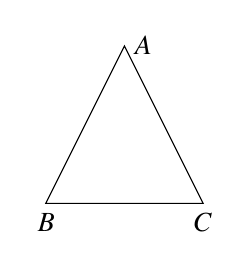
\begin{tikzpicture}
\draw (0,0) node[anchor=north]{$B$}
  -- (1,2) node[anchor=west]{$A$}
  -- (2,0) node[anchor=north]{$C$}
  -- cycle;
\end{tikzpicture}
%}
%\end{document}
%\section{Quadrilateral}
%\renewcommand{\theequation}{\theenumi}
%\begin{enumerate}[label=\arabic*.,ref=\thesection.\theenumi]
%\numberwithin{equation}{enumi}
	%
%
\item Construct parallelogram $ABCD$ 	in Fig. \ref{fig:pgm_sas}	
given that  $BC = 5, AB = 6, \angle C = 85 \degree$.
\begin{figure}[!ht]
	\begin{center}
		\resizebox{\columnwidth}{!}{%Code by GVV Sharma
%December 10, 2019
%released under GNU GPL
%Drawing a parallelogram given 2 sides and an angle

\begin{tikzpicture}
[scale=2,>=stealth,point/.style={draw,circle,fill = black,inner sep=0.5pt},]

%Triangle sides
\def\a{5}
\def\b{6}
\def\c{7.467975323683154}
%Coordinates of D
%\def\p{{\a^2+\c^2-\b^2}/{(2*\a)}}
\def\p{4.477065543514051}
\def\q{{sqrt(\c^2-\p^2)}}

%Labeling points
\node (D) at (\p,\q)[point,label=above right:$D$] {};
\node (B) at (0, 0)[point,label=below left:$B$] {};
\node (C) at (\a, 0)[point,label=below right:$C$] {};
\node (O) at ($(B)!0.5!(D)$)[point,label=below right:$O$] {};

%Coordinates of A

\node (A) at ($(O)!-1!(C)$)[point,label=above right:$A$] {};


%Drawing parallelogram ABCD
\draw (A) -- (B) --  (C) --(D)--(A);
\draw (A) -- (C);
\draw (B) --(D);


\tkzMarkAngle[fill=green!20](C,A,D)
\tkzMarkAngle[fill=green!20](A,C,B)
%
%
\tkzMarkAngle[fill=red!30](A,D,B)
\tkzMarkAngle[fill=red!30](C,B,D)


\tkzMarkAngle[fill=orange!40](D,C,O)
\tkzMarkAngle[fill=orange!40](B,A,C)

\tkzMarkAngle[fill=blue!50](B,D,C)
\tkzMarkAngle[fill=blue!50](D,B,A)

\end{tikzpicture}
}
	\end{center}
	\caption{Parallelogram Properties}
	\label{fig:pgm_sas}	
\end{figure}
%
\\
\solution $BD$ is found using the cosine formula and $\triangle BDC$ is drawn using the approach in Construction \ref{const:tri_sss} with 
%
\begin{align}
\vec{B} = \myvec{0\\0},
\vec{C} = \myvec{5\\0},
\end{align}
%
Since the diagonals bisect each other, 
%
\begin{align}
\vec{O} &= \frac{\vec{B}+\vec{D}}{2}
\\
\vec{A} &= 2\vec{O} - \vec{C}.
\end{align}
%
$AB$ and $AD$ are then joined to complete the $\parallel$gm.
The python code for  Fig. \ref{fig:pgm_sas} is
\begin{lstlisting}
codes/quad/pgm_sas.py
\end{lstlisting}
%
and 
The equivalent latex-tikz code is
%
\begin{lstlisting}
figs/quad/pgm_sas.tex
\end{lstlisting}
%

\item Draw the $\parallel$gm $ABCD$ in 	Fig. \ref{fig:pgm_sss}	
with $BC = 6, CD = 4.5$ and $BD=7.5$.  Show that it is a rectangle.
\label{const:pgm_sss}
%
\begin{figure}[!ht]
	\begin{center}
		\resizebox{\columnwidth}{!}{%Code by GVV Sharma
%December 12, 2019
%released under GNU GPL
%Drawing a rectangle given two sides

\begin{tikzpicture}
[scale=2,>=stealth,point/.style={draw,circle,fill = black,inner sep=0.5pt},]

%Triangle sides
\def\a{6}
\def\b{4.5}
%\def\c{7.5}

%Labeling points
\node (D) at (\a,\b)[point,label=above right:$D$] {};
\node (B) at (0, 0)[point,label=below left:$B$] {};
\node (C) at (\a, 0)[point,label=below right:$C$] {};
\node (A) at (0,\b)[point,label=right:$A$] {};
\node (O) at ($(B)!0.5!(D)$)[point,label=right:$O$] {};

%A



%Drawing parallelogram ABCD
\draw (A) -- (B) --  (C) --(D)--(A);
\draw (A) -- (C);
\draw (B) --(D);


\tkzMarkRightAngle[fill=blue!20,size=.2](B,C,D)

%
\end{tikzpicture}
}
	\end{center}
	\caption{Rectangle}
	\label{fig:pgm_sss}	
\end{figure}
\\
\solution It is easy to verify that 
%Using the approach in Construction\ref{const:tri_sss}, $\triangle BCD$ is drawn with
%
\begin{align}
BD^2=BC^2+C^2
\end{align}
%
Hence, using Baudhayana theorem, 
%
\begin{align}
\angle BCD = 90\degree
\end{align}
%
and  $ABCD$ is a rectangle.
\begin{align}
\vec{A} = \myvec{0\\4.5}
\vec{B} = \myvec{0\\0}
\vec{C} = \myvec{6\\0}
\vec{D} = \myvec{6\\4}
\end{align}
%
The python code for  Fig. \ref{fig:pgm_sss} is
\begin{lstlisting}
codes/quad/pgm_sss.py
\end{lstlisting}
%
and the equivalent latex-tikz code is
%
\begin{lstlisting}
figs/quad/pgm_sss.tex
\end{lstlisting}
%
%
%
%
%
\item Draw the rhombus $BEST$ with $BE = 4.5$ and $ET = 6$. 
\begin{figure}[!ht]
	\begin{center}
		\resizebox{\columnwidth}{!}{%Code by GVV Sharma
%December 10, 2019
%released under GNU GPL
%Drawing a rhombus given a side and a diagonal

\begin{tikzpicture}
[scale=2,>=stealth,point/.style={draw,circle,fill = black,inner sep=0.5pt},]

%Triangle sides
\def\a{4.5}%BE
\def\b{6}%ET
\def\p{\b/2}%OE
\def\q{{sqrt(\a^2-\p^2)}}%OB

%Labeling points
\node (B) at (0,-\q)[point,label=below :$B$] {};
\node (E) at (\p, 0)[point,label=right:$E$] {};
\node (S) at (0, \q)[point,label=above:$S$] {};
\node (T) at (-\p,0)[point,label=left:$T$] {};
\node (O) at (0, 0)[point,label=below left:$O$] {};


%Drawing parallelogram ABCD
\draw (B) -- (E) --  (S) --(T)--(B);
\draw (B) -- (S);
\draw (E) --(T);


\tkzMarkRightAngle[fill=blue!20,size=.2](B,O,E)

%
\end{tikzpicture}
}
	\end{center}
	\caption{Rhombus}
	\label{fig:rhom_sss}	
\end{figure}
\\
\solution The coordinates of the various points in Fig. \ref{fig:rhom_sss} are obtained as
%
\begin{align}
\vec{O} = \myvec{0\\0},
\vec{B} = \myvec{0\\-4.5}
\\
\vec{E} = \myvec{3\\0},
\vec{S} = \myvec{4.5\\0},
\vec{T} = \myvec{0\\-3}
\end{align}
%
\item A square is a rectangle whose sides are equal.  Draw a square of side 4.5.
\\
\solution The coordinates of the various points in Fig. \ref{fig:square} are obtained as
%
\begin{align}
\vec{A} = \myvec{0\\4.5}
\\
\vec{B} = \myvec{0\\0},
\vec{C} = \myvec{4.5\\0},
\vec{D} = \myvec{4.5\\4.5}
\vec{O} = \frac{\vec{B}+\vec{C}}{2}
%
\end{align}
%
\begin{figure}[!ht]
	\begin{center}
		\resizebox{\columnwidth}{!}{%Code by GVV Sharma
%December 12, 2019
%released under GNU GPL
%Drawing a square given a side 

\begin{tikzpicture}
[scale=2,>=stealth,point/.style={draw,circle,fill = black,inner sep=0.5pt},]

%Square side
\def\a{4.5}

%Labeling points
\node (A) at (0,\a)[point,label=below :$A$] {};
\node (B) at (0,0)[point,label=below :$B$] {};
\node (C) at (\a, 0)[point,label=right:$C$] {};
\node (D) at (\a, \a)[point,label=above:$D$] {};
\node (O) at ($(B)!0.5!(D)$)[point,label=below left:$O$] {};


%Drawing square ABCD
\draw (A) -- (B) --  (C) --(D)--(A);
\draw (B) -- (D);
\draw (A) --(C);


\tkzMarkRightAngle[fill=blue!20,size=.2](C,O,D)
\tkzMarkRightAngle[fill=blue!20,size=.2](A,B,C)

%
\end{tikzpicture}
}
	\end{center}
	\caption{Square}
	\label{fig:square}	
\end{figure}

%
%\end{enumerate}

\end{enumerate}

\section{Exercises}
\renewcommand{\theequation}{\theenumi}
\begin{enumerate}[label=\thesection.\arabic*.,ref=\thesection.\theenumi]
\numberwithin{equation}{enumi}
\renewcommand{\theequation}{\theenumi}
\begin{enumerate}[label=\thesection.\arabic*.,ref=\thesection.\theenumi]
%\begin{enumerate}[label=\arabic*.,ref=\thesection.\theenumi]
\numberwithin{equation}{enumi}

\item Construct a triangle of sides $a=4$, $b=5$  and $c=6$.  
\item Construct an isosceles triangle whose base is $a=8$cm and altitude $AD=h=4$cm 
\item In $\triangle ABC$,  given that $a+b+c = 11, \angle B = 45^{\degree}$ and $\angle C = 45^{\degree}$, 
find 
$a,b,c$ and sketch the triangle.
\item Draw $\triangle ABC$ with $a = 6, c = 5$ and $\angle B = 60 \degree$. 
\item Draw $\triangle ABC$ with $a = 7, \angle B = 45\degree$ and $\angle A = 105 \degree$. 
\item $\triangle ABC$ is right angled at $\vec{B}$.  If $a = 12$ and $b+c = 18$, find $b,c$ and draw the triangle.
%\item Draw $\triangle ABC$ if $AB = 3, AC = 5$ and $\angle C = 30 \degree$.
\item In $\triangle ABC$,  $a = 8, \angle B = 45^{\degree}$ and $c-b = 3.5$.
Sketch $\triangle ABC$.

\item In $\triangle ABC$,  $a = 6, \angle B = 60^{\degree}$ and $b-c = 2$. 
Sketch $\triangle ABC$.
\item Draw $\triangle ABC$,  given that $a+b+c = 11, \angle B = 30^{\degree}$ and $\angle C = 90^{\degree}$.
\item Construct $\triangle xyz$ where $xy = 4.5, yz = 5$ and $zx = 6$.
\item Draw an equilateral triangle of side $5.5$.
\item Draw $\triangle PQR$ with $PQ = 4, QR = 3.5$ and $PR = 4$.  What type of triangle is this?
\item Construct $\triangle ABC$ such that $AB = 2.5, BC = 6$ and $AC = 6.5$.  Find $\angle B$.
\item Construct $\triangle PQR$, given that $PQ = 3, QR = 5.5$ and $\angle PQR = 60 \degree$.
\item Construct $\triangle DEF$ such that $DE = 5, DF = 3$ and $\angle D = 90\degree$.
\item Construct an isosceles triangle in which the lengths of the equal sides is 6.5 and the angle between them is $110\degree$.
\item Construct $\triangle ABC$  with $BC = 7.5, AC = 5$ and $\angle C = 60\degree$.
\item Construct $\triangle XYZ$ if $XY = 6, \angle X = 30\degree$ and $\angle Y = 100 \degree$.
\item If $AC = 7, \angle A = 60\degree$ and $\angle B = 50 \degree$, can you draw the triangle?
\item Construct $\triangle ABC$ given that $\angle A = 60\degree, \angle B = 30\degree$ and $AB = 5.8$.
\item Construct $\triangle PQR$ if $PQ = 5, \angle Q = 105 \degree$ and $\angle R = 40 \degree$.
\item Can you construct $\triangle DEF$ such that $EF = 7.2, \angle E = 110\degree$ and $\angle F = 180\degree$?
\item Construct  $\triangle LMN$ right angled at $M$ such that $LN = 5$ and $MN = 3$.
\item Construct  $\triangle PQR$ right angled at $Q$ such that $QR = 8$ and $PR = 10$.
\item Construct  right angled $\triangle $ whose hypotenuse  is 6 and one of the legs is 4.
\item Construct  an isosceles right angled $\triangle ABC$ right angled at $C$ such $AC = 6$.
\item Construct the  triangles in Table \ref{table:triangle_const_exercises}.
\begin{table}[!ht]
%%%%%%%%%%%%%%%%%%%%%%%%%%%%%%%%%%%%%%%%%%%%%%%%%%%%%%%%%%%%%%%%%%%%%%
%%                                                                  %%
%%  This is the header of a LaTeX2e file exported from Gnumeric.    %%
%%                                                                  %%
%%  This file can be compiled as it stands or included in another   %%
%%  LaTeX document. The table is based on the longtable package so  %%
%%  the longtable options (headers, footers...) can be set in the   %%
%%  preamble section below (see PRAMBLE).                           %%
%%                                                                  %%
%%  To include the file in another, the following two lines must be %%
%%  in the including file:                                          %%
%%        \def\inputGnumericTable{}                                 %%
%%  at the beginning of the file and:                               %%
%%        \input{name-of-this-file.tex}                             %%
%%  where the table is to be placed. Note also that the including   %%
%%  file must use the following packages for the table to be        %%
%%  rendered correctly:                                             %%
%%    \usepackage[latin1]{inputenc}                                 %%
%%    \usepackage{color}                                            %%
%%    \usepackage{array}                                            %%
%%    \usepackage{longtable}                                        %%
%%    \usepackage{calc}                                             %%
%%    \usepackage{multirow}                                         %%
%%    \usepackage{hhline}                                           %%
%%    \usepackage{ifthen}                                           %%
%%  optionally (for landscape tables embedded in another document): %%
%%    \usepackage{lscape}                                           %%
%%                                                                  %%
%%%%%%%%%%%%%%%%%%%%%%%%%%%%%%%%%%%%%%%%%%%%%%%%%%%%%%%%%%%%%%%%%%%%%%



%%  This section checks if we are begin input into another file or  %%
%%  the file will be compiled alone. First use a macro taken from   %%
%%  the TeXbook ex 7.7 (suggestion of Han-Wen Nienhuys).            %%
\def\ifundefined#1{\expandafter\ifx\csname#1\endcsname\relax}


%%  Check for the \def token for inputed files. If it is not        %%
%%  defined, the file will be processed as a standalone and the     %%
%%  preamble will be used.                                          %%
\ifundefined{inputGnumericTable}

%%  We must be able to close or not the document at the end.        %%
	\def\gnumericTableEnd{\end{document}}


%%%%%%%%%%%%%%%%%%%%%%%%%%%%%%%%%%%%%%%%%%%%%%%%%%%%%%%%%%%%%%%%%%%%%%
%%                                                                  %%
%%  This is the PREAMBLE. Change these values to get the right      %%
%%  paper size and other niceties.                                  %%
%%                                                                  %%
%%%%%%%%%%%%%%%%%%%%%%%%%%%%%%%%%%%%%%%%%%%%%%%%%%%%%%%%%%%%%%%%%%%%%%

	\documentclass[12pt%
			  %,landscape%
                    ]{report}
       \usepackage[latin1]{inputenc}
       \usepackage{fullpage}
       \usepackage{color}
       \usepackage{array}
       \usepackage{longtable}
       \usepackage{calc}
       \usepackage{multirow}
       \usepackage{hhline}
       \usepackage{ifthen}

	\begin{document}


%%  End of the preamble for the standalone. The next section is for %%
%%  documents which are included into other LaTeX2e files.          %%
\else

%%  We are not a stand alone document. For a regular table, we will %%
%%  have no preamble and only define the closing to mean nothing.   %%
    \def\gnumericTableEnd{}

%%  If we want landscape mode in an embedded document, comment out  %%
%%  the line above and uncomment the two below. The table will      %%
%%  begin on a new page and run in landscape mode.                  %%
%       \def\gnumericTableEnd{\end{landscape}}
%       \begin{landscape}


%%  End of the else clause for this file being \input.              %%
\fi

%%%%%%%%%%%%%%%%%%%%%%%%%%%%%%%%%%%%%%%%%%%%%%%%%%%%%%%%%%%%%%%%%%%%%%
%%                                                                  %%
%%  The rest is the gnumeric table, except for the closing          %%
%%  statement. Changes below will alter the table's appearance.     %%
%%                                                                  %%
%%%%%%%%%%%%%%%%%%%%%%%%%%%%%%%%%%%%%%%%%%%%%%%%%%%%%%%%%%%%%%%%%%%%%%

\providecommand{\gnumericmathit}[1]{#1} 
%%  Uncomment the next line if you would like your numbers to be in %%
%%  italics if they are italizised in the gnumeric table.           %%
%\renewcommand{\gnumericmathit}[1]{\mathit{#1}}
\providecommand{\gnumericPB}[1]%
{\let\gnumericTemp=\\#1\let\\=\gnumericTemp\hspace{0pt}}
 \ifundefined{gnumericTableWidthDefined}
        \newlength{\gnumericTableWidth}
        \newlength{\gnumericTableWidthComplete}
        \newlength{\gnumericMultiRowLength}
        \global\def\gnumericTableWidthDefined{}
 \fi
%% The following setting protects this code from babel shorthands.  %%
 \ifthenelse{\isundefined{\languageshorthands}}{}{\languageshorthands{english}}
%%  The default table format retains the relative column widths of  %%
%%  gnumeric. They can easily be changed to c, r or l. In that case %%
%%  you may want to comment out the next line and uncomment the one %%
%%  thereafter                                                      %%
\providecommand\gnumbox{\makebox[0pt]}
%%\providecommand\gnumbox[1][]{\makebox}

%% to adjust positions in multirow situations                       %%
\setlength{\bigstrutjot}{\jot}
\setlength{\extrarowheight}{\doublerulesep}

%%  The \setlongtables command keeps column widths the same across  %%
%%  pages. Simply comment out next line for varying column widths.  %%
\setlongtables

\setlength\gnumericTableWidth{%
	10pt+%
	32pt+%
	45pt+%
	45pt+%
	45pt+%
	0pt+%
0pt}
\def\gumericNumCols{6}
\setlength\gnumericTableWidthComplete{\gnumericTableWidth+%
         \tabcolsep*\gumericNumCols*2+\arrayrulewidth*\gumericNumCols}
\ifthenelse{\lengthtest{\gnumericTableWidthComplete > \linewidth}}%
         {\def\gnumericScale{\ratio{\linewidth-%
                        \tabcolsep*\gumericNumCols*2-%
                        \arrayrulewidth*\gumericNumCols}%
{\gnumericTableWidth}}}%
{\def\gnumericScale{1}}

%%%%%%%%%%%%%%%%%%%%%%%%%%%%%%%%%%%%%%%%%%%%%%%%%%%%%%%%%%%%%%%%%%%%%%
%%                                                                  %%
%% The following are the widths of the various columns. We are      %%
%% defining them here because then they are easier to change.       %%
%% Depending on the cell formats we may use them more than once.    %%
%%                                                                  %%
%%%%%%%%%%%%%%%%%%%%%%%%%%%%%%%%%%%%%%%%%%%%%%%%%%%%%%%%%%%%%%%%%%%%%%

\ifthenelse{\isundefined{\gnumericColA}}{\newlength{\gnumericColA}}{}\settowidth{\gnumericColA}{\begin{tabular}{@{}p{10pt*\gnumericScale}@{}}x\end{tabular}}
\ifthenelse{\isundefined{\gnumericColB}}{\newlength{\gnumericColB}}{}\settowidth{\gnumericColB}{\begin{tabular}{@{}p{32pt*\gnumericScale}@{}}x\end{tabular}}
\ifthenelse{\isundefined{\gnumericColC}}{\newlength{\gnumericColC}}{}\settowidth{\gnumericColC}{\begin{tabular}{@{}p{45pt*\gnumericScale}@{}}x\end{tabular}}
\ifthenelse{\isundefined{\gnumericColD}}{\newlength{\gnumericColD}}{}\settowidth{\gnumericColD}{\begin{tabular}{@{}p{45pt*\gnumericScale}@{}}x\end{tabular}}
\ifthenelse{\isundefined{\gnumericColE}}{\newlength{\gnumericColE}}{}\settowidth{\gnumericColE}{\begin{tabular}{@{}p{45pt*\gnumericScale}@{}}x\end{tabular}}
\ifthenelse{\isundefined{\gnumericColF}}{\newlength{\gnumericColF}}{}\settowidth{\gnumericColF}{\begin{tabular}{@{}p{24pt*\gnumericScale}@{}}x\end{tabular}}

\begin{tabular}[c]{%
	b{\gnumericColA}%
	b{\gnumericColB}%
	b{\gnumericColC}%
	b{\gnumericColD}%
	b{\gnumericColE}%
	b{\gnumericColF}%
	}

%%%%%%%%%%%%%%%%%%%%%%%%%%%%%%%%%%%%%%%%%%%%%%%%%%%%%%%%%%%%%%%%%%%%%%
%%  The longtable options. (Caption, headers... see Goosens, p.124) %%
%	\caption{The Table Caption.}             \\	%
% \hline	% Across the top of the table.
%%  The rest of these options are table rows which are placed on    %%
%%  the first, last or every page. Use \multicolumn if you want.    %%

%%  Header for the first page.                                      %%
%	\multicolumn{6}{c}{The First Header} \\ \hline 
%	\multicolumn{1}{c}{colTag}	%Column 1
%	&\multicolumn{1}{c}{colTag}	%Column 2
%	&\multicolumn{1}{c}{colTag}	%Column 3
%	&\multicolumn{1}{c}{colTag}	%Column 4
%	&\multicolumn{1}{c}{colTag}	%Column 5
%	&\multicolumn{1}{c}{colTag}	\\ \hline %Last column
%	\endfirsthead

%%  The running header definition.                                  %%
%	\hline
%	\multicolumn{6}{l}{\ldots\small\slshape continued} \\ \hline
%	\multicolumn{1}{c}{colTag}	%Column 1
%	&\multicolumn{1}{c}{colTag}	%Column 2
%	&\multicolumn{1}{c}{colTag}	%Column 3
%	&\multicolumn{1}{c}{colTag}	%Column 4
%	&\multicolumn{1}{c}{colTag}	%Column 5
%	&\multicolumn{1}{c}{colTag}	\\ \hline %Last column
%	\endhead

%%  The running footer definition.                                  %%
%	\hline
%	\multicolumn{6}{r}{\small\slshape continued\ldots} \\
%	\endfoot

%%  The ending footer definition.                                   %%
%	\multicolumn{6}{c}{That's all folks} \\ \hline 
%	\endlastfoot
%%%%%%%%%%%%%%%%%%%%%%%%%%%%%%%%%%%%%%%%%%%%%%%%%%%%%%%%%%%%%%%%%%%%%%

\hhline{|-|-|---~}
	 \multicolumn{1}{|p{\gnumericColA}|}%
	{\gnumericPB{\centering}\gnumbox{\textbf{S.No}}}
	&\multicolumn{1}{p{\gnumericColB}|}%
	{\gnumericPB{\centering}\gnumbox{\textbf{Triangle }}}
	&\multicolumn{3}{p{	\gnumericColC+%
	\gnumericColD+%
	\gnumericColE+%
	\tabcolsep*2*2}|}%
	{\gnumericPB{\centering}\gnumbox{\textbf{Given Measurements}}}
	&
\\
\hhline{|---|-|-|~}
	 \multicolumn{1}{|p{\gnumericColA}|}%
	{\gnumericPB{\centering}\gnumbox{1}}
	&\multicolumn{1}{p{\gnumericColB}|}%
	{\gnumericPB{\centering}\gnumbox{$\triangle$ABC}}
	&\multicolumn{1}{p{\gnumericColC}|}%
	{\gnumericPB{\raggedright}\gnumbox[l]{$\angle A=85\degree$}}
	&\multicolumn{1}{p{\gnumericColD}|}%
	{\gnumericPB{\raggedright}\gnumbox[l]{ $\angle B=115 \degree$ }}
	&\multicolumn{1}{p{\gnumericColE}|}%
	{\gnumericPB{\raggedright}\gnumbox[l]{AB = 5 }}
	&
\\
\hhline{|-----|~}
	 \multicolumn{1}{|p{\gnumericColA}|}%
	{\gnumericPB{\centering}\gnumbox{2}}
	&\multicolumn{1}{p{\gnumericColB}|}%
	{\gnumericPB{\centering}\gnumbox{$\triangle$PQR}}
	&\multicolumn{1}{p{\gnumericColC}|}%
	{\gnumericPB{\raggedright}\gnumbox[l]{$\angle Q=30 \degree$}}
	&\multicolumn{1}{p{\gnumericColD}|}%
	{\gnumericPB{\raggedright}\gnumbox[l]{$\angle R=60 \degree$}}
	&\multicolumn{1}{p{\gnumericColE}|}%
	{\gnumericPB{\raggedright}\gnumbox[l]{QR = 4.7 }}
	&
\\
\hhline{|-----|~}
	 \multicolumn{1}{|p{\gnumericColA}|}%
	{\gnumericPB{\centering}\gnumbox{3}}
	&\multicolumn{1}{p{\gnumericColB}|}%
	{\gnumericPB{\centering}\gnumbox{$\triangle$ABC}}
	&\multicolumn{1}{p{\gnumericColC}|}%
	{\gnumericPB{\raggedright}\gnumbox[l]{$\angle A=70 \degree$}}
	&\multicolumn{1}{p{\gnumericColD}|}%
	{\gnumericPB{\raggedright}\gnumbox[l]{$\angle B=50 \degree$}}
	&\multicolumn{1}{p{\gnumericColE}|}%
	{\gnumericPB{\raggedright}\gnumbox[l]{AC = 3 }}
	&
\\
\hhline{|-----|~}
	 \multicolumn{1}{|p{\gnumericColA}|}%
	{\gnumericPB{\centering}\gnumbox{4}}
	&\multicolumn{1}{p{\gnumericColB}|}%
	{\gnumericPB{\centering}\gnumbox{$\triangle$LMN}}
	&\multicolumn{1}{p{\gnumericColC}|}%
	{\gnumericPB{\raggedright}\gnumbox[l]{$\angle L=60 \degree$  }}
	&\multicolumn{1}{p{\gnumericColD}|}%
	{\gnumericPB{\raggedright}\gnumbox[l]{$\angle N=120 \degree$}}
	&\multicolumn{1}{p{\gnumericColE}|}%
	{\gnumericPB{\raggedright}\gnumbox[l]{LM = 5 }}
	&
\\
\hhline{|-----|~}
	 \multicolumn{1}{|p{\gnumericColA}|}%
	{\gnumericPB{\centering}\gnumbox{5}}
	&\multicolumn{1}{p{\gnumericColB}|}%
	{\gnumericPB{\centering}\gnumbox{$\triangle$ABC}}
	&\multicolumn{1}{p{\gnumericColC}|}%
	{\gnumericPB{\raggedright}\gnumbox[l]{BC = 2  }}
	&\multicolumn{1}{p{\gnumericColD}|}%
	{\gnumericPB{\raggedright}\gnumbox[l]{AB = 4 }}
	&\multicolumn{1}{p{\gnumericColE}|}%
	{\gnumericPB{\raggedright}\gnumbox[l]{AC = 2 }}
	&
\\
\hhline{|-----|~}
	 \multicolumn{1}{|p{\gnumericColA}|}%
	{\gnumericPB{\centering}\gnumbox{6}}
	&\multicolumn{1}{p{\gnumericColB}|}%
	{\gnumericPB{\centering}\gnumbox{$\triangle$PQR}}
	&\multicolumn{1}{p{\gnumericColC}|}%
	{\gnumericPB{\raggedright}\gnumbox[l]{PQ = 2.5 }}
	&\multicolumn{1}{p{\gnumericColD}|}%
	{\gnumericPB{\raggedright}\gnumbox[l]{ QR = 4  }}
	&\multicolumn{1}{p{\gnumericColE}|}%
	{\gnumericPB{\raggedright}\gnumbox[l]{PR = 3.5 }}
	&
\\
\hhline{|-----|~}
	 \multicolumn{1}{|p{\gnumericColA}|}%
	{\gnumericPB{\centering}\gnumbox{7}}
	&\multicolumn{1}{p{\gnumericColB}|}%
	{\gnumericPB{\centering}\gnumbox{$\triangle$XYZ}}
	&\multicolumn{1}{p{\gnumericColC}|}%
	{\gnumericPB{\raggedright}\gnumbox[l]{XY = 3   }}
	&\multicolumn{1}{p{\gnumericColD}|}%
	{\gnumericPB{\raggedright}\gnumbox[l]{YZ = 4 }}
	&\multicolumn{1}{p{\gnumericColE}|}%
	{\gnumericPB{\raggedright}\gnumbox[l]{XZ = 5 }}
	&
\\
\hhline{|-----|~}
	 \multicolumn{1}{|p{\gnumericColA}|}%
	{\gnumericPB{\centering}\gnumbox{8}}
	&\multicolumn{1}{p{\gnumericColB}|}%
	{\gnumericPB{\centering}\gnumbox{$\triangle$DEF}}
	&\multicolumn{1}{p{\gnumericColC}|}%
	{\gnumericPB{\raggedright}\gnumbox[l]{DE = 4.5  }}
	&\multicolumn{1}{p{\gnumericColD}|}%
	{\gnumericPB{\raggedright}\gnumbox[l]{EF = 5.5 }}
	&\multicolumn{1}{p{\gnumericColE}|}%
	{\gnumericPB{\raggedright}\gnumbox[l]{DF = 4 }}
	&
\\
\hhline{|-|-|-|-|-|~}
\end{tabular}

\ifthenelse{\isundefined{\languageshorthands}}{}{\languageshorthands{\languagename}}
\gnumericTableEnd

\caption{}
\label{table:triangle_const_exercises}
\end{table}

\end{enumerate}
%

\renewcommand{\theequation}{\theenumi}
\begin{enumerate}[label=\thesubsection.\arabic*.,ref=\thesubsection.\theenumi]
%\begin{enumerate}[label=\arabic*.,ref=\thesection.\theenumi]
\numberwithin{equation}{enumi}


\item Construct a quadrilateral $ABCD$ such that $AB=5, \angle A = 50\degree, AC = 4, BD = 5$ and $AD = 6$.
\item Construct $PQRS$ where $PQ = 4, QR = 6, RS = 5, PS = 5.5$ and $PR = 7$.
\item Draw $JUMP$ with $JU = 3.5, UM=4, MP = 5, PJ =4.5$ and $PU = 6.5$
\item Construct a quadrilateral $ABCD$ such that $BC=4.5,  AC = 5.5, CD = 5, BD = 7$ and $AD = 5.5$.
\item Can you construct a quadrilateral $PQRS$ with $PQ=3, RS=3, PS=7.5, PR=8$ and $SQ=4$?
\item Construct $LIFT$ such that $LI = 4, IF = 3, TL = 2.5, LF = 4.5, IT=4$.
\item Draw $GOLD$ such that $OL=7.5, GL=6, GD=6, LD = 5, OD = 10$.
\item DRAW rhombus $BEND$ such that $BN = 5.6$, $DE = 6.5$.
\item construct a quadrilateral MIST where $MI = 3.5, IS = 6.5, \angle M = 75 \degree, \angle I = 105 \degree$ and $\angle S = 120 \degree$.
\item Can you construct the above quadrilateral MIST if $\angle M = 100 \degree$ instead of $75 \degree$.
\item Can you constrcut the quadrilateral PLAN if $PL = 6, LA = 9.5, \angle P = 75 \degree, \angle L = 150 \degree$ and $\angle A = 140 \degree$?
\item Construct $MORE$ where $MO = 6, OR = 4.5, \angle M = 60 \degree, \angle O = 105 \degree, \angle R = 105 \degree$.
\item Construct $PLAN$ where $PL = 4, LA = 6.5, \angle P = 90 \degree, \angle A = 110\degree$ and $\angle N = 85\degree$.
\item Draw  rectangle $OKAY$ with $OK = 7$ and $KA = 5$.
\item Construct $ABCD $, where $AB = 4, BC = 5, Cd = 6.5, \angle B = 105 \degree$ and $\angle C = 80\degree$.
\item Construct $DEAR$ with $DE = 4, EA = 5, AR = 4.5, \angle E = 60 \degree$ and $\angle A = 90 \degree$.\item Construct $TRUE$ with $TR = 3.5, RU = 3, UE = 4 \angle R = 75\degree$ and $\angle U = 120\degree$.

\item Can you construct a rhombus $ABCD$ with $AC = 6$ and $BD = 7$?
\item Draw a square $READ$ with $RE = 5.1$.
\item Draw a rhombus who diagonals are $5.2$ and $6.4$.
\item Draw a rectangle with adjacent sides $5$ and $4$.
\item Draw a parallelogram $OKAY$ with $OK = 5.5$ and $KA = 4.2$.
\item Construct a kite $EASY$ if $AY = 8, EY = 4$ and $SY = 6$.


\end{enumerate}
%

%\renewcommand{\theequation}{\theenumi}
%\begin{enumerate}[label=\thesubsection.\arabic*.,ref=\thesubsection.\theenumi]
%%\begin{enumerate}[label=\arabic*.,ref=\thesection.\theenumi]
%\numberwithin{equation}{enumi}

\item Draw a circle of diameter 6.1

\item With the same centre $\vec{O}$,  draw two circles of radii 4 and 2.5
\item Draw a circle with centre $\vec{B}$ and radius 6.  If $\vec{C}$ be  a point 10 units  away from its 
centre, construct the pair of tangents $AC$ and $CD$ to the 
circle.
\item Draw a circle of radius 3 and any two of its diameters.  Draw the ends of these diameters. What figure do you get?
\item Let $\vec{A}$ and $\vec{B}$ be the centres of two circles of equal radii 3 such that each one of them passes through the centre of the other.  Let them intersect at $\vec{C}$ and $\vec{D}$.  Is $AB \perp CD$?

\item Construct a tangent to a circle of radius 4 units from a point on the concentric circle of radius 6 
units.
\\
\solution Take the centre of both circles to be at the origin.  
\item Draw a circle of radius 3 units. Take  two points $\vec{P}$ and $\vec{Q}$ on one of its extended 
diameter each at a distance of 7 units from its centre. Draw tangents to the circle from these two points 
$\vec{P}$ and $\vec{Q}$.
\\
\solution Take the diameter to be on the $x$-axis.
\item Draw a pair of tangents to a circle of radius 5 units which are inclined to each other at an angle of 
$60^{\degree}$.
\\
\solution The tangent is perpendicular to the radius.
\item Draw a line segment $AB$ of length 8 units. Taking $\vec{A}$ as centre, draw a circle of radius 4 units 
and taking $\vec{B}$ as centre, draw another circle of radius 3 units. Construct tangents to each circle from 
the centre of the other circle.
\\
\solution Let
\begin{align}
\vec{A} = \myvec{0 \\ 0}, \vec{B} = \myvec{8 \\ 0}.
\end{align}
\item Let ABC be a right triangle in which $a = 8, c = 6$ and $\angle B = 90^{\degree}$.  $BD$ is the 
perpendicular from $\vec{B}$ on $AC$ (altitude). The circle through $\vec{B}, \vec{C}, \vec{D}$ (circumcircle of $\triangle BCD$) is drawn.  Construct the 
tangents from $\vec{A}$ to this circle.
%\\
%\solution Since $\angle BDC = 90\degree$, $BC$ is the diameter of the circumcircle of $\triangle BCD$. Since $AB \perp BC$ and $BC$ is the diameter, $AB$ is a tangent to the circumcircle of $\triangle BCD$.  Let $\vec{O}$ be the centre of the circle.  The point of contact is obtained by rotating $\vec{B}$ by $\theta = 2\angle BAO$. Thus, if 
%\begin{align}
%\vec{B} &= \myvec{0 \\ 0}, \vec{C} = \myvec{a \\ 0},
%\\
%\vec{O} &= \frac{1}{2}\myvec{a \\ 0}
%\end{align}

\item Draw a circle with centre $\vec{C}$ and radius 3.4.  Draw any chord.  Construct the perpendicular bisector of the chord and examine if it passes through $\vec{C}$
%\end{enumerate}
%
%\item Form the differential equation represeting the family of curves given by 
%\begin{align}
%\vec{x}^T \myvec{1 & 0 \\ 0 & 2} \vec{x} -\myvec{2a & 0}\vec{x} = 0,
%\end{align}
%%
%where $a$ is an arbitrary constant.
%%
%\item Form the differntial equation of the family of circles in the first quadrant which touch the coordinate axes.
%\end{enumerate}

%\section{Quadrilateral}
%%\renewcommand{\theequation}{\theenumi}
%\begin{enumerate}[label=\arabic*.,ref=\thesection.\theenumi]
%\numberwithin{equation}{enumi}
	%
%
\item Construct parallelogram $ABCD$ 	in Fig. \ref{fig:pgm_sas}	
given that  $BC = 5, AB = 6, \angle C = 85 \degree$.
\begin{figure}[!ht]
	\begin{center}
		\resizebox{\columnwidth}{!}{%Code by GVV Sharma
%December 10, 2019
%released under GNU GPL
%Drawing a parallelogram given 2 sides and an angle

\begin{tikzpicture}
[scale=2,>=stealth,point/.style={draw,circle,fill = black,inner sep=0.5pt},]

%Triangle sides
\def\a{5}
\def\b{6}
\def\c{7.467975323683154}
%Coordinates of D
%\def\p{{\a^2+\c^2-\b^2}/{(2*\a)}}
\def\p{4.477065543514051}
\def\q{{sqrt(\c^2-\p^2)}}

%Labeling points
\node (D) at (\p,\q)[point,label=above right:$D$] {};
\node (B) at (0, 0)[point,label=below left:$B$] {};
\node (C) at (\a, 0)[point,label=below right:$C$] {};
\node (O) at ($(B)!0.5!(D)$)[point,label=below right:$O$] {};

%Coordinates of A

\node (A) at ($(O)!-1!(C)$)[point,label=above right:$A$] {};


%Drawing parallelogram ABCD
\draw (A) -- (B) --  (C) --(D)--(A);
\draw (A) -- (C);
\draw (B) --(D);


\tkzMarkAngle[fill=green!20](C,A,D)
\tkzMarkAngle[fill=green!20](A,C,B)
%
%
\tkzMarkAngle[fill=red!30](A,D,B)
\tkzMarkAngle[fill=red!30](C,B,D)


\tkzMarkAngle[fill=orange!40](D,C,O)
\tkzMarkAngle[fill=orange!40](B,A,C)

\tkzMarkAngle[fill=blue!50](B,D,C)
\tkzMarkAngle[fill=blue!50](D,B,A)

\end{tikzpicture}
}
	\end{center}
	\caption{Parallelogram Properties}
	\label{fig:pgm_sas}	
\end{figure}
%
\\
\solution $BD$ is found using the cosine formula and $\triangle BDC$ is drawn using the approach in Construction \ref{const:tri_sss} with 
%
\begin{align}
\vec{B} = \myvec{0\\0},
\vec{C} = \myvec{5\\0},
\end{align}
%
Since the diagonals bisect each other, 
%
\begin{align}
\vec{O} &= \frac{\vec{B}+\vec{D}}{2}
\\
\vec{A} &= 2\vec{O} - \vec{C}.
\end{align}
%
$AB$ and $AD$ are then joined to complete the $\parallel$gm.
The python code for  Fig. \ref{fig:pgm_sas} is
\begin{lstlisting}
codes/quad/pgm_sas.py
\end{lstlisting}
%
and 
The equivalent latex-tikz code is
%
\begin{lstlisting}
figs/quad/pgm_sas.tex
\end{lstlisting}
%

\item Draw the $\parallel$gm $ABCD$ in 	Fig. \ref{fig:pgm_sss}	
with $BC = 6, CD = 4.5$ and $BD=7.5$.  Show that it is a rectangle.
\label{const:pgm_sss}
%
\begin{figure}[!ht]
	\begin{center}
		\resizebox{\columnwidth}{!}{%Code by GVV Sharma
%December 12, 2019
%released under GNU GPL
%Drawing a rectangle given two sides

\begin{tikzpicture}
[scale=2,>=stealth,point/.style={draw,circle,fill = black,inner sep=0.5pt},]

%Triangle sides
\def\a{6}
\def\b{4.5}
%\def\c{7.5}

%Labeling points
\node (D) at (\a,\b)[point,label=above right:$D$] {};
\node (B) at (0, 0)[point,label=below left:$B$] {};
\node (C) at (\a, 0)[point,label=below right:$C$] {};
\node (A) at (0,\b)[point,label=right:$A$] {};
\node (O) at ($(B)!0.5!(D)$)[point,label=right:$O$] {};

%A



%Drawing parallelogram ABCD
\draw (A) -- (B) --  (C) --(D)--(A);
\draw (A) -- (C);
\draw (B) --(D);


\tkzMarkRightAngle[fill=blue!20,size=.2](B,C,D)

%
\end{tikzpicture}
}
	\end{center}
	\caption{Rectangle}
	\label{fig:pgm_sss}	
\end{figure}
\\
\solution It is easy to verify that 
%Using the approach in Construction\ref{const:tri_sss}, $\triangle BCD$ is drawn with
%
\begin{align}
BD^2=BC^2+C^2
\end{align}
%
Hence, using Baudhayana theorem, 
%
\begin{align}
\angle BCD = 90\degree
\end{align}
%
and  $ABCD$ is a rectangle.
\begin{align}
\vec{A} = \myvec{0\\4.5}
\vec{B} = \myvec{0\\0}
\vec{C} = \myvec{6\\0}
\vec{D} = \myvec{6\\4}
\end{align}
%
The python code for  Fig. \ref{fig:pgm_sss} is
\begin{lstlisting}
codes/quad/pgm_sss.py
\end{lstlisting}
%
and the equivalent latex-tikz code is
%
\begin{lstlisting}
figs/quad/pgm_sss.tex
\end{lstlisting}
%
%
%
%
%
\item Draw the rhombus $BEST$ with $BE = 4.5$ and $ET = 6$. 
\begin{figure}[!ht]
	\begin{center}
		\resizebox{\columnwidth}{!}{%Code by GVV Sharma
%December 10, 2019
%released under GNU GPL
%Drawing a rhombus given a side and a diagonal

\begin{tikzpicture}
[scale=2,>=stealth,point/.style={draw,circle,fill = black,inner sep=0.5pt},]

%Triangle sides
\def\a{4.5}%BE
\def\b{6}%ET
\def\p{\b/2}%OE
\def\q{{sqrt(\a^2-\p^2)}}%OB

%Labeling points
\node (B) at (0,-\q)[point,label=below :$B$] {};
\node (E) at (\p, 0)[point,label=right:$E$] {};
\node (S) at (0, \q)[point,label=above:$S$] {};
\node (T) at (-\p,0)[point,label=left:$T$] {};
\node (O) at (0, 0)[point,label=below left:$O$] {};


%Drawing parallelogram ABCD
\draw (B) -- (E) --  (S) --(T)--(B);
\draw (B) -- (S);
\draw (E) --(T);


\tkzMarkRightAngle[fill=blue!20,size=.2](B,O,E)

%
\end{tikzpicture}
}
	\end{center}
	\caption{Rhombus}
	\label{fig:rhom_sss}	
\end{figure}
\\
\solution The coordinates of the various points in Fig. \ref{fig:rhom_sss} are obtained as
%
\begin{align}
\vec{O} = \myvec{0\\0},
\vec{B} = \myvec{0\\-4.5}
\\
\vec{E} = \myvec{3\\0},
\vec{S} = \myvec{4.5\\0},
\vec{T} = \myvec{0\\-3}
\end{align}
%
\item A square is a rectangle whose sides are equal.  Draw a square of side 4.5.
\\
\solution The coordinates of the various points in Fig. \ref{fig:square} are obtained as
%
\begin{align}
\vec{A} = \myvec{0\\4.5}
\\
\vec{B} = \myvec{0\\0},
\vec{C} = \myvec{4.5\\0},
\vec{D} = \myvec{4.5\\4.5}
\vec{O} = \frac{\vec{B}+\vec{C}}{2}
%
\end{align}
%
\begin{figure}[!ht]
	\begin{center}
		\resizebox{\columnwidth}{!}{%Code by GVV Sharma
%December 12, 2019
%released under GNU GPL
%Drawing a square given a side 

\begin{tikzpicture}
[scale=2,>=stealth,point/.style={draw,circle,fill = black,inner sep=0.5pt},]

%Square side
\def\a{4.5}

%Labeling points
\node (A) at (0,\a)[point,label=below :$A$] {};
\node (B) at (0,0)[point,label=below :$B$] {};
\node (C) at (\a, 0)[point,label=right:$C$] {};
\node (D) at (\a, \a)[point,label=above:$D$] {};
\node (O) at ($(B)!0.5!(D)$)[point,label=below left:$O$] {};


%Drawing square ABCD
\draw (A) -- (B) --  (C) --(D)--(A);
\draw (B) -- (D);
\draw (A) --(C);


\tkzMarkRightAngle[fill=blue!20,size=.2](C,O,D)
\tkzMarkRightAngle[fill=blue!20,size=.2](A,B,C)

%
\end{tikzpicture}
}
	\end{center}
	\caption{Square}
	\label{fig:square}	
\end{figure}

%
%\end{enumerate}

\end{enumerate}

%
\end{document}


